% Chapter 3

\chapter{CHAPTER THREE\\3.0 METHODOLOGY} % Main chapter title

\label{Chapter3} % For referencing the chapter elsewhere, use \ref{Chapter1} 

%-----------------------------------------------------------------------------------

\section{Introduction}
The techniques used to study our model are outlined in this chapter, together with a comprehensive explanation of the mathematical tools and constructs, theorems, lemmas, and their justifications.  The planning and execution processes of our technique make use of the R programming language. During the planning process, we considered where to get our data from and the procedures needed to build a time series model from the satellite data. We categorize our research as taking a quantitative approach. This research is specifically a causal-comparative experimental study with the goal of identifying the variability climate is responsible for in vegetation loss in Ghana.
 \section{Study Area}
 The Republic of Ghana, a nation in West Africa, will serve as the location for the experimental plots for this study. It shares borders with the Ivory Coast in the west, Burkina Faso in the north, and Togo in the east. It borders the Gulf of Guinea and the Atlantic Ocean to the south. Ghana's total size is 238,535 km2 (92,099 sq mi), and it is made up of a variety of biomass, from tropical rain forests to coastal savannas. Ghana, which has a population of over 31 million, is the second-most populous nation in West Africa, behind Nigeria.Accra, the nation's capital and largest city, as well as Kumasi, Tamale, and Sekondi-Takoradi, are other important cities
\begin{figure}
	\centering
	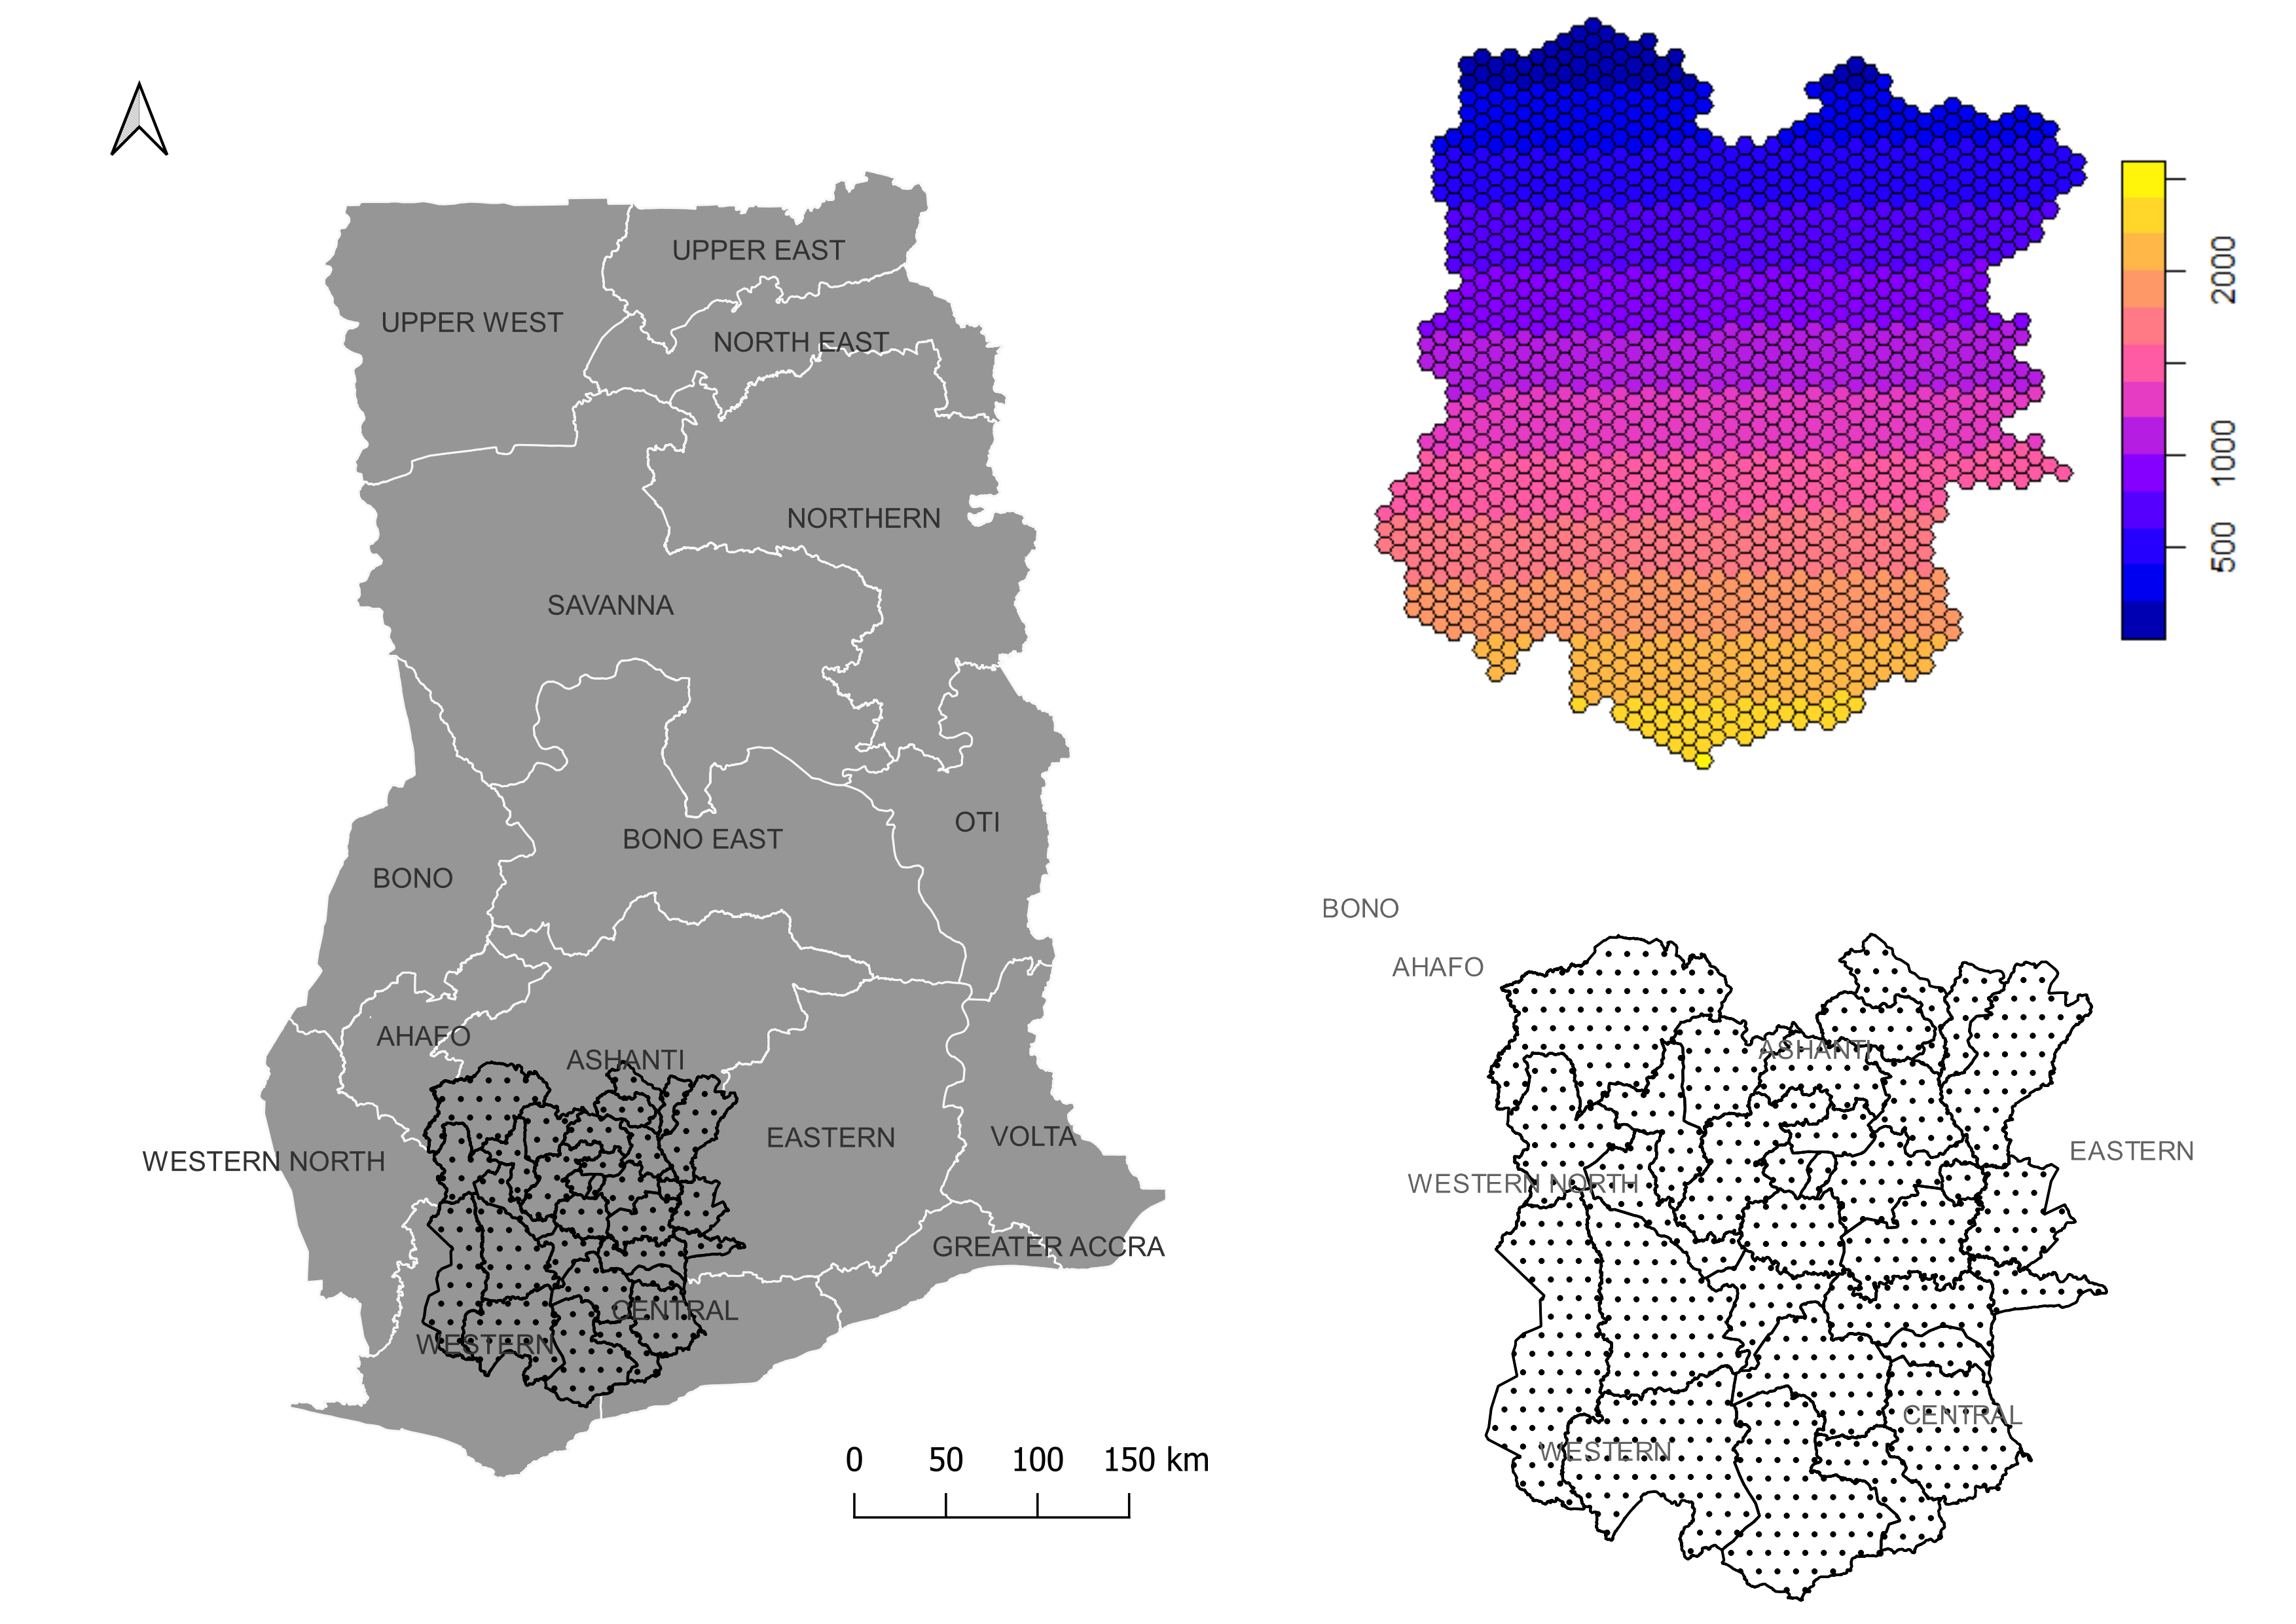
\includegraphics[width=0.9\linewidth]{images/StudyArea}
	\caption{Study Area}
	\label{fig:studyarea}
\end{figure}
\section{DATA }
Data gathering. The majority of the quantitative data came from the Ghana Meteorological Agency and the Health Service. Rainfall, the highest temperature, and relative humidity are some of the meteorological data that were measured from 2010 to 2015 on a mean monthly basis. Additionally, based on monthly incidences for the Kumasi Metropolitan Area from 2000 to 2022, the data for EVI were obtained.

\subsection{Data Description and Inspection}

Data from a time series is a set of observations made in a particular order over a period of time. There is a chance for correlation between observations because time series data points are gathered at close intervals. To help machine learning classifiers work with time series data, we provide several new tools. We first contend that local features or patterns in time series can be found and combined to address challenges involving time-series categorization. Then, a method to discover patterns that are helpful for classification is suggested. We combine these patterns to create computable categorization rules. In order to mask low-quality pixels, we will first collect data from Google Earth Engine in order to choose  EVI values and Climate Change data.

Instead of analyzing the imagery directly, we will summarize the mean  Climate values. This will shorten the analysis time while still providing an attractive and useful map. We will apply a smoothing strategy using an ARIMA function to fix the situation where some cells may not have  EVI for a particular month. Once NA values have been eliminated, the time series will be divided to eliminate seasonality before the normalized data is fitted using a linear model. We will go to classify our data on the map and map it after we have extracted the linear trend.

Here, we made sure that we checked our data set for missing values and discovered there were none. The dataset’s number of columns is shown in the table below,
which also details the counts and datatype of various features in our dataset. No values are missing when there is a count of 133990. Anything below that denotes
the existence of unreported values.


 \subsection{Time Series Forecasting Using Stochastic Models}
 The selection of a proper model is extremely important as it reflects the underlying structure of the series and this fitted model in turn is
 used for future forecasting. A time series model is said to be linear or non-linear depending on whether the current value of the series is a
 linear or non-linear function of past observations.
 
 In general models for time series data can have many forms and represent different stochastic processes. There are two widely used linear time series models in literature.
 
 \emph{Autoregressive (AR)} and \emph{Moving Average (MA)} models, combining these two, the Autoregressive Moving Average (ARMA) and  \emph{Autoregressive Integrated Moving Average (ARIMA)} models have been proposed in many literature. The \emph{Autoregressive Fractionally Integrated Moving Average (ARFIMA)} model generalizes ARMA and ARIMA models. For seasonal time series forecasting, a variation of ARIMA. The  \emph{Seasonal Autoregressive Integrated Moving Average (SARIMA)}  model is used.
 
 ARIMA model and its different variations are based on the famous Box-Jenkins principle Hipel and McLeod \parencite{hipel1994time} and so these are also broadly known as the Box-Jenkins models.
\textbf{Vector Autoregression Model}\\
Model of vector autoregression. In econometrics, the Sims' vector autoregression (VAR) model has been widely employed to analyze multivariate time series. It provides better forecasting abilities than a univariate time series model and is a logical extension of the univariate autoregressive model to dynamic multivariate time series. Additionally, it identifies how each endogenous variable responds over time to a shock in both its own value and in every other variable. This method also enables the researcher to follow the data. The VAR model of order $p$ Sims \parencite{sims1980macroeconomics} proposed has the following basic form:
\begin{equation}
	y_{t} = A_{1}y_{t-1} + A_{2}y_{t-2} +\cdot+A_{p}y_{t-p}+ CD_{t} + \mu 
\end{equation}
Where $ y_{t} = \left( y_{1t},y_{2t},...,y_{kt}\right)'$ is a vector of K observable endogenous variables. For the purposes of this study, yt = $(EVI_{t}, Temperature_{t}, Rain_{}, Precipitation_{t},Drought_{t},Evaporation_{t})'$ where EVI denotes the value of vegetation conditions  each month, Temperature for both TMax and TMin, Rain denotes the amount of precipitation (mm), and Drought denotes the relative drought (\%). All deterministic variables, including constants, linear trends, and seasonal dummy variables, are contained in $CD_{t}$. An unobservable zero-mean white noise process in K dimensions, $\mu_{t}$ has a positive definite covariance matrix $E(\mu_{t},\mu_{t}^{'}) = \sum_{\mu}$. We  apply different limits on the parameter matrices $A_{i}$ and C, which are of an appropriate dimension.
Generalized least squares is used to estimate the model's parameters.

\textbf{Augmented Dickey Fuller Test.} For stationarity, detecting the presence of a unit root in quite general time series models. Our approach is nonparametric with respect to nuisance parameters and thereby allows for a very wide class of weakly dependent and possibly heterogeneously distributed data. The tests accommodate models with a fitted drift and a time trend so that they may be used to discriminate between unit root nonstationarity and stationarity about a deterministic trend. The limiting distributions of the statistics are obtained under both the unit root null and a sequence of local alternatives. The latter noncentral distribution theory yields local asymptotic power functions for the tests and facilitates comparisons with alternative procedures due to Dickey \& Fuller \parencite{phillips1988testing}.

\begin{align}        \Delta y_t &=  \gamma y_{t-1} + \underbrace{\sum_{i=2}^{p} \beta_i \Delta y_{t-i+1}}_\text{control for serial correlation} + \epsilon_t  \\ \rightarrow (\tau1&)\quad H_0 :  {\gamma = 0} \\\\       \Delta y_t &=  {\gamma} y_{t-1}  + \underbrace{{a_0}}_\text{constant} + \sum_{i=2}^{p} \beta_i \Delta y_{t-i+1} + \epsilon_t   \\ \rightarrow (\phi1&)\quad H_0 :  {\gamma = 0} \quad\&\quad{a_0 = 0}  \\\ \rightarrow (\tau2&)\quad H_0 :  {\gamma = 0}  \\\       \Delta y_t &=  {\gamma} y_{t-1}  + {a_0}  + \underbrace{{a_2} t}_{trend} + \sum_{i=2}^{p} \beta_i \Delta y_{t-i+1}  + \epsilon_t \\ \rightarrow (\phi2&)\quad H_0 :  {\gamma = 0} \quad\&\quad {a_0 = 0} \quad\&\quad {a_2 = 0} \\ \rightarrow (\phi3&)\quad H_0 :  {\gamma = 0} \quad\&\quad{a_0 = 0}  \\ \rightarrow (\tau3&)\quad H_0 :  {\gamma = 0}    
 \end{align}
 \textbf{(ADF)} test is a unit root test. The alternative hypothesis varies slightly depending on the equation used, whereas the null hypothesis for the ADF test is that there is a unit root. The time series is steady, which is the most straightforward alternate theory. In time series analysis, unit roots can lead to unexpected outcomes.\\

\textbf{Optimal Lag Length Selection Criteria (OLS)}  is used to estimate each of the system's individual equations. One of the following Information Criteria is minimized to determine the best lag order that is choosing optimal lag  to reduce residual correlation
\begin{center}
		\begin{tabular}{ll}
			\multicolumn{1}{c}{}Criteria &  Formular \\ \midrule
			Akaike Information Criterion,AIC (n)  & = log det $ \displaystyle\left(\sum _{\mu}(n)\right)+ \frac{2}{T}nK^{2}$\\
			Hannan-Quinn criterion,HQ(n)    & = log det  $ \displaystyle\left(\sum _{\mu}(n)\right)+ \frac{2logT}{T}nK^{2}$\\
			Schwarz Criterion,SC(n)    & = log det  $ \displaystyle\left(\sum _{\mu}(n)\right)+ \frac{logT}{T}nK^{2}$\\
			Final Prediction Error criterion,FPE(n)   & =          $\displaystyle \left(\frac{T + n^{*}}{T - n^{*}}\right)$det $\displaystyle \left(\sum_{\mu}(n)\right)$\\ \bottomrule
		\end{tabular}
\end{center}
where $ \displaystyle \sum_{\mu} (n)$ is the estimated by $T^{-1}\sum_{t=1}^{T}$
\section{Structural Analysis}
There are frequently many coefficients to comprehend, despite the fact that VAR coefficients describe the projected impact of a variable. Examining the model's residuals, which represent unforeseen contemporaneous events, is typically more prevalent. The next subsections explain some of the typical methods used for structural analysis of VAR models in a manner that is comparatively nontechnical.
\subsection{Causality Analysis} Both the Granger-causality and instantaneous causality were investigated. For both tests, the vector of endogenous variables is divided into two subvectors,$y_{1t}$ and $y_{2t}$ with dimensions $K_{1}$ and $K_{2}$,ctively, so that $K = K_{1} + K_{2}$ The subvector $y_{1t}$ said to be Granger-causal for
$y_{2t}$ if the past of $y_{1t}$ significantly helps predicting the future of $y_{2t}$ a the past of $y_{1t}$ one \parencite{granger1969investigating}. For testing this property,
a model of the form
\begin{equation}
	\displaystyle
	\left[ \begin{array}{c} y_{1t} \\ y_{2t}  \end{array} \right] \mbox{=} \sum_{i=1}^{p}\left[\begin{array}{cc}
		\alpha_{11,i} & \alpha_{12,i} \\
		\alpha_{21,i} & \alpha_{22,i} 
	\end{array}
\right]
\left[\begin{array}{c}
		y_{1,t-i}\\
		y_{2,t-i}
	\end{array}\right] + CD_{t} + \left[ \begin{array}{c}
		\mu_{1t}\\
		\mu_{2t}
	\end{array}\right]
\end{equation}
Where, $y_{1t}$ is not considered as  Granger-causal for $y_{2t}$ if and only if $ \alpha_{21,i} = 0,$ i = 1,2,...p.
Therefore, this null hypothesis is tested that at least one of the $\alpha_{21,i}$, has a positive value. The constraints are tested using an F-test statistic with a distribution of $F(pK_{1}K_{2}, KT - n^{*})$. Here, $n^{*}$ is the entire number of system parameters, including those for the deterministic term \parencite{lutkepohl2005new}. To test Granger-cause from $y_{2t}$ to $y_{1t}$, the roles of $y_{1t}$ and $y_{2t}$ can be switched.In other words, Granger causality responds to the question of whether previous values of the variable x may help anticipate future values of the variable y.

Instantaneous causality is defined as having a nonzero correlation between $\mu_{1t}$ and $\mu_{2t}$. Consequently, the null hypothesis is tested against the alternative 
\begin{equation}
	H_{0}: E\left(\mu_{1t},\mu_{2t}^{'} \right)
\end{equation}
is checked for instantaneous causation versus the alternative of nonzero covariance between the two error vectors. This hypothesis is investigated using a Wald test statistic.
\textbf{Analysis of impulse responses}: Exogenous and deterministic variables are viewed as fixed in impulse response analysis and can thus be removed from the system. Now, $y_{t}$ stands for the adjusted endogenous variables. The process $y_{t}$ has a Wold moving average (MA) representation if it is stationary \textbf{(I(0))}, which is represented by 
\begin{equation}
	y_{t} = \varPhi_{0}\mu_{t} + \varPhi_{1}\mu_{t-1} + \varPhi_{2}\mu_{t-2} + \dots
\end{equation}
Where $\varPhi_{0} =I_{K}$ and the $\varPhi_{s}$ can be computed recursively as 
\begin{equation}
	\varPhi_{s} = \sum_{j=i}^{s}\varPhi_{s-j}A_{j}, \quad s = 1,2,\dots,
\end{equation}
With $\varPhi = I_{K}$ and $A_{j} = 0 $ for $j>p$. The coefficients of this
representation may be interpreted as reflecting the responses
to impulses hitting the system. The \emph{(i,j)th} element of the matrices $\varPhi_{s},$ regarded as a function of \emph{s}, trace out the expected
response of $y_{i,t+s}$ to a unit change in $y_{it}$ holding constant all
past values of $y_{t}$
\section{ Forecast Error Variance Decomposition}
Denoting the $(i,j)th$ element of the orthogonalized impulse response
coefcient matrix $\theta_{n}$ by $\theta_{ij,n}$, the variance of the forecast error $\left(y_{k,T+h}-y_{k,T+h|T}\right)$ is 
\begin{equation}
	\begin{split}
		\displaystyle
		\sigma^{2}_{k}(h) & = \sum^{h-1}_{n=0}\left(\theta^{2}_{k1,n} + \cdot+ \theta^{2}_{kK,n}\right) \\
		& =\sum^{K}_{j=1}\left(\theta^{2}_{kj,0} + \cdot+ \theta^{2}_{kj,h=1}\right)
	\end{split}
\end{equation}
The term $\displaystyle \left(\theta^{2}_{kj,0} + \cdot+ \theta^{2}_{kj,h=1}\right) $ is interpreted as the contribution
of variable \emph{j} to the \emph{h}-step forecast error variance of variable
\emph{k}.  Dividing the above terms by $\displaystyle \sigma^{2}_{k}(h)$ gives the percentage \emph{j} to the \emph{h}-step forecast error variance of variable
\emph{k}, 
\begin{equation}
	\omega_{kj}(h) =\frac{\left(\theta^{2}_{kj,0} + \cdot+ \theta^{2}_{kj,h=1}\right)}{\sigma^{2}_{k}(h)}
\end{equation}
\section{Forecast Performance Measures}

While applying a particular model to some real or simulated time series, first the raw data is divided into two parts (\textbf{Training Set and
	Test Set}). The observations in the training set are used for constructing the desired model. Often a small sub-part of the training
set is kept for validation purpose and is known as the \textbf{Validation Set}. Sometimes a preprocessing is done by normalizing the data or taking logarithmic or other transforms. One such famous technique is the Box-Cox Transformation {[}23{]}. Once a model is constructed, it is used for generating forecasts. The test set observations are kept for verifying how accurate the fitted model performed in forecasting these values. If necessary, an inverse transformation is applied on the forecast values to convert them in original scale. In order to judge the forecasting accuracy of a particular model or for evaluating and comparing different models, their relative performance on the test dataset is considered.

Due to the fundamental importance of time series forecasting in many practical situations, proper care should be taken while selecting a particular model. For this reason, various performance measures are proposed in literature to estimate forecast accuracy and to compare different models. These are also known as performance metrics {[}24{]}. Each of these measures is a function of the actual and forecast values of the time series.

% this line fixes the vertical padding of text inside the cells
%\renewcommand{\arraystretch}{1.4}
%\begin{sidewaystable}
%	\caption{Description of Various Forecast Performance Measures}
%	\label{tab:my-table}
%	\resizebox{\columnwidth}{2.5cm}
%	\begin{tabularx}{\textwidth}{|L{2cm}|X|L{2cm}|L{2cm}|X|}{lllll}
%		\hline
%		& \multicolumn{4}{l}{\cellcolor[HTML]{C0C0C0}}{Error Matrix} \\ \midrule    
%		
%		& \multicolumn{1}{l}{MAE}
%		& \multicolumn{1}{l}{RMSE}
%		& \multicolumn{1}{l}{MSE}
%		& \multicolumn{1}{l}{MAPE} \\
%		\midrule
%		\multicolumn{13}{l}{}                                \\
%		\\\multicolumn{13}{l}{}   \\ 
%		
%		\multicolumn{13}{c}{Where: In each of the forthcoming definitions, $y_{t }$ is the actual value,$f_{t}$ is the forecast value, $e_{t} = y_{t} - f_{t}$ is the forecast error and n is the size of the test set. Also, $\displaystyle \bar{y} = \frac{1}{n}\sum_{t=1}^{n}y_{t}$ is the test mean and $\displaystyle \sigma^{2} = \frac{1}{n-1}\sum_{t=1}^{n}(y_{t}-\bar{y})^{2}$is the test variance.}                                \\\hline\hline
%		Formulas 
%		& $\displaystyle MAE = \frac{1}{n}\sum_{t=1}^{n}|e_{t}|$ \\
%		& $\displaystyle RMSE = \sqrt{MSE} = \sqrt {\frac{1}{n}\sum_{t=1}^{n}e^{2}_{t}}$ \\
%		& $\displaystyle MSE = \frac{1}{n}\sum_{t=1}^{n}e^{2}_{t}$\\
%		& $\displaystyle MAPE= \frac{1}{n}\sum^{n}\left(\frac{e_{t}}{y_{t}}\right)$ \\ \bottomrule
%		
%		\multicolumn{13}{l}{}                                \\
%	\end{tabularx}%
%	
%	
%\end{sidewaystable}

\subsection{Description of Various Forecast Performance Measures}
\textbf{MAPE}\\
This measure represents the percentage of average absolute error occurred. It is independent of the scale of measurement, but affected by data transformation.It does not show the direction of error. MAPE does not penalize extreme deviations. In this measure, opposite signed errors do not offset each other.
\\
\textbf{MSE}\\
It is a measure of average squared deviation of forecast values. As here the opposite signed errors do not offset one another, MSE gives an overall idea of the error occurred during forecasting. It penalizes extreme errors occurred while forecasting. MSE emphasizes the fact that the total forecast error is in fact much   affected by large individual errors, i.e. large errors are much expensive than small errors. MSE does not provide any idea about the direction of overall error. MSE is sensitive to the change of scale and data transformations. Although MSE is a good measure of overall forecast error, but it is   not as intuitive and easily interpretable as the other measures discussed before. 

\textbf{RMSE}\\
RMSE is nothing but the square root of calculated MSE. All the properties of MSE hold for RMSE as well.

\textbf{MAD}\\
measures the average absolute deviation of forecast values from   original ones.It shows the magnitude of overall error, occurred due to forecasting.In MAE, the effects of positive and negative errors do not cancel out.Unlike MFE, MAE does not provide any idea about the direction of  errors. For a good forecast, the obtained MAE should be as small as possible. Like MFE, MAE also depends on the scale of measurement and data   transformations.Extreme forecast errors are not panelized by MAE.\\
%\begin{landscape}
	\begin{table}[]
		\label{table:Performance Measures}
		\caption{Various Forecast Performance Measures}
		\centering
		\addtolength{\tabcolsep}{30pt}
		\begin{tabularx}{\textwidth}{@{}llll@{}}
			\toprule \hline
			MAE	&  RMSE   &  MSE   &  MAPE  \\ \midrule
			
			$\displaystyle  \frac{1}{n}\sum_{t=1}^{n}|e_{t}|$	& $\displaystyle  \sqrt{MSE} = \sqrt {\frac{1}{n}\sum_{t=1}^{n}e^{2}_{t}}$    & $\displaystyle  \frac{1}{n}\sum_{t=1}^{n}e^{2}_{t}$    & $\displaystyle  \frac{1}{n}\sum^{n}\left(\frac{e_{t}}{y_{t}}\right)$   \\ \bottomrule
			
		\end{tabularx}
	\end{table}
%\end{landscape}
Where: In each of the forthcoming definitions, $y_{t }$ is the actual value,$f_{t}$ is the forecast value, $e_{t} = y_{t} - f_{t}$ is the forecast error and n is the size of the test set. Also, $\displaystyle \bar{y} = \frac{1}{n}\sum_{t=1}^{n}y_{t}$ is the test mean and $\displaystyle \sigma^{2} = \frac{1}{n-1}\sum_{t=1}^{n}(y_{t}-\bar{y})^{2}$is the test variance.

